\section{String Pallindrome}
\subsection{Aim}
To check whether a string is pallindrome

\subsection{Code}
\begin{lstlisting}
DATA SEGMENT
    str DB 'abba$'
    strlen EQU $-str
    pallindromes DB 'pallindrome$'
    notpallindromes DB 'not pallindrome$'
DATA ENDS

CODE SEGMENT
ASSUME CS:CODE, DS:DATA
START:
    MOV AX, DATA
    MOV DS, AX
    LEA SI, str
    LEA DI, str
    ADD DI, strlen
    SUB DI, 2 
    MOV CX, strlen
    SUB CX, 2

COMP:
    MOV AL, [DI]
    CMP AL, [SI]
    JNE NOTPALLINDROME
    INC SI
    DEC DI
    LOOP COMP

OUTPUT:   
    LEA DX, pallindromes
    MOV AH, 09H
    INT 21H
    JMP EXIT
    
NOTPALLINDROME:
    LEA DX, notpallindromes
    MOV AH, 09H
    INT 21H
    
EXIT:
    MOV AH, 4CH
    INT 21H
CODE ENDS
END START

\end{lstlisting}

\subsection{Output}
\begin{center}
	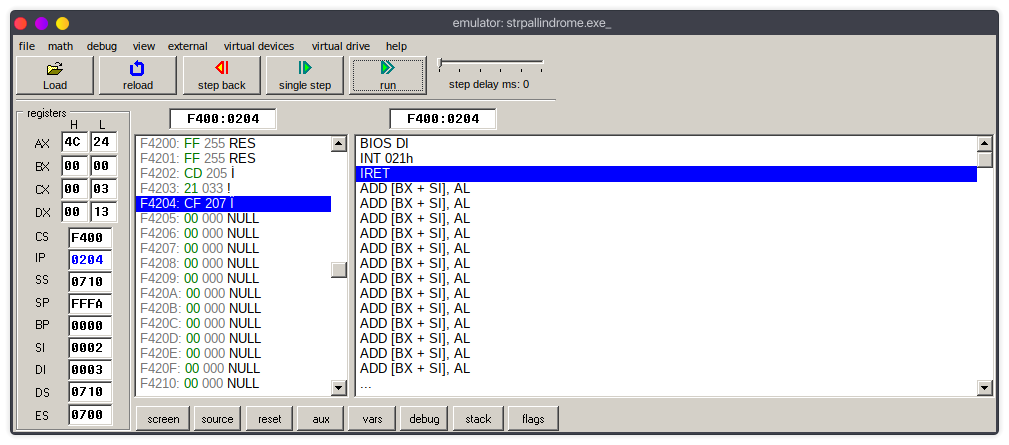
\includegraphics[width=0.90\textwidth]{img/p17/ss1.png}
	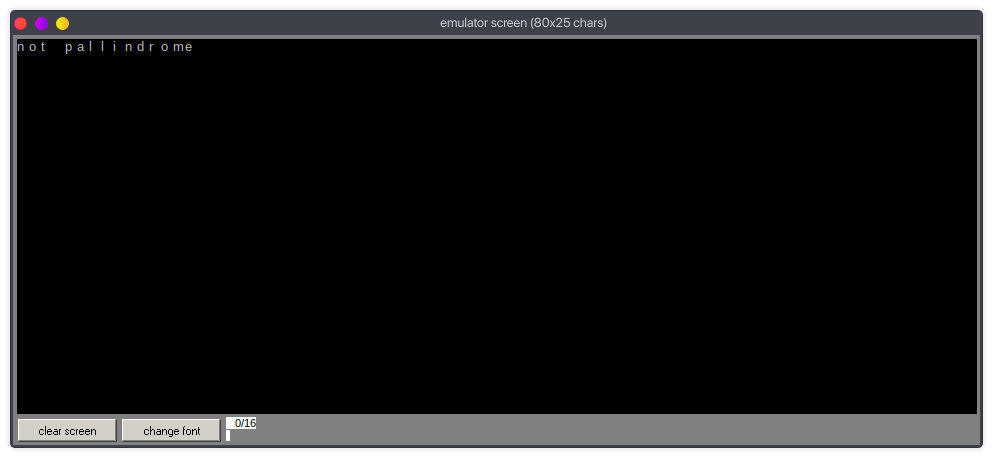
\includegraphics[width=0.90\textwidth]{img/p17/ss2.png}\\
    Output for abcdba\\

    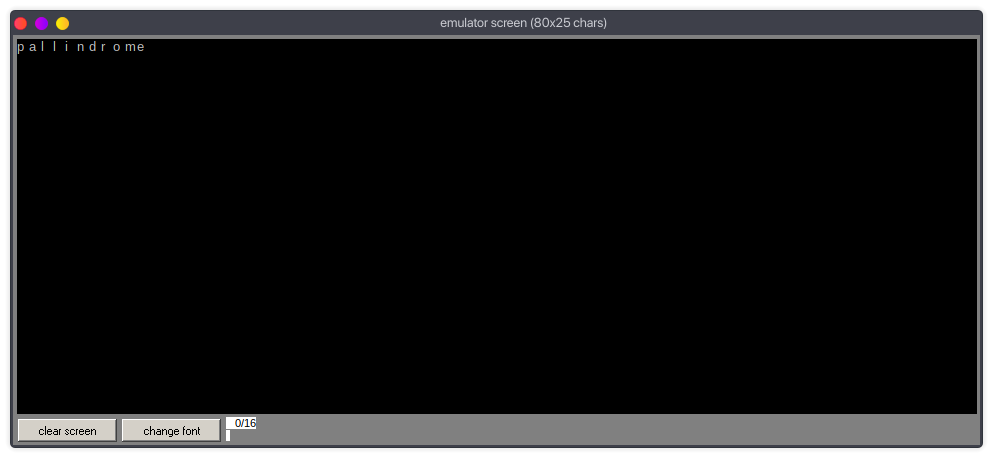
\includegraphics[width=0.90\textwidth]{img/p17/ss3.png}\\
    Output for abccba\\
\end{center}

\subsection{Result}
A string is checked to be pallindrome or not

